\newpage
\section{OSINT}

\subsection{The meeting (40p)}
The counter intelligence captured a message that is flagged as suspicious. ``Let's meet tomorrow at \texttt{///pens.ferrets.cages} at 10. I'll give you all documents.'' Can you help them to find out where the meeting takes place?

\textbf{Solution:}\\
I found this task a bit difficult mostly because i didn't understand what the three slashes ment. So I searched for the cages suffix assuming it was a file extension, and stumbled upon what3words.com.

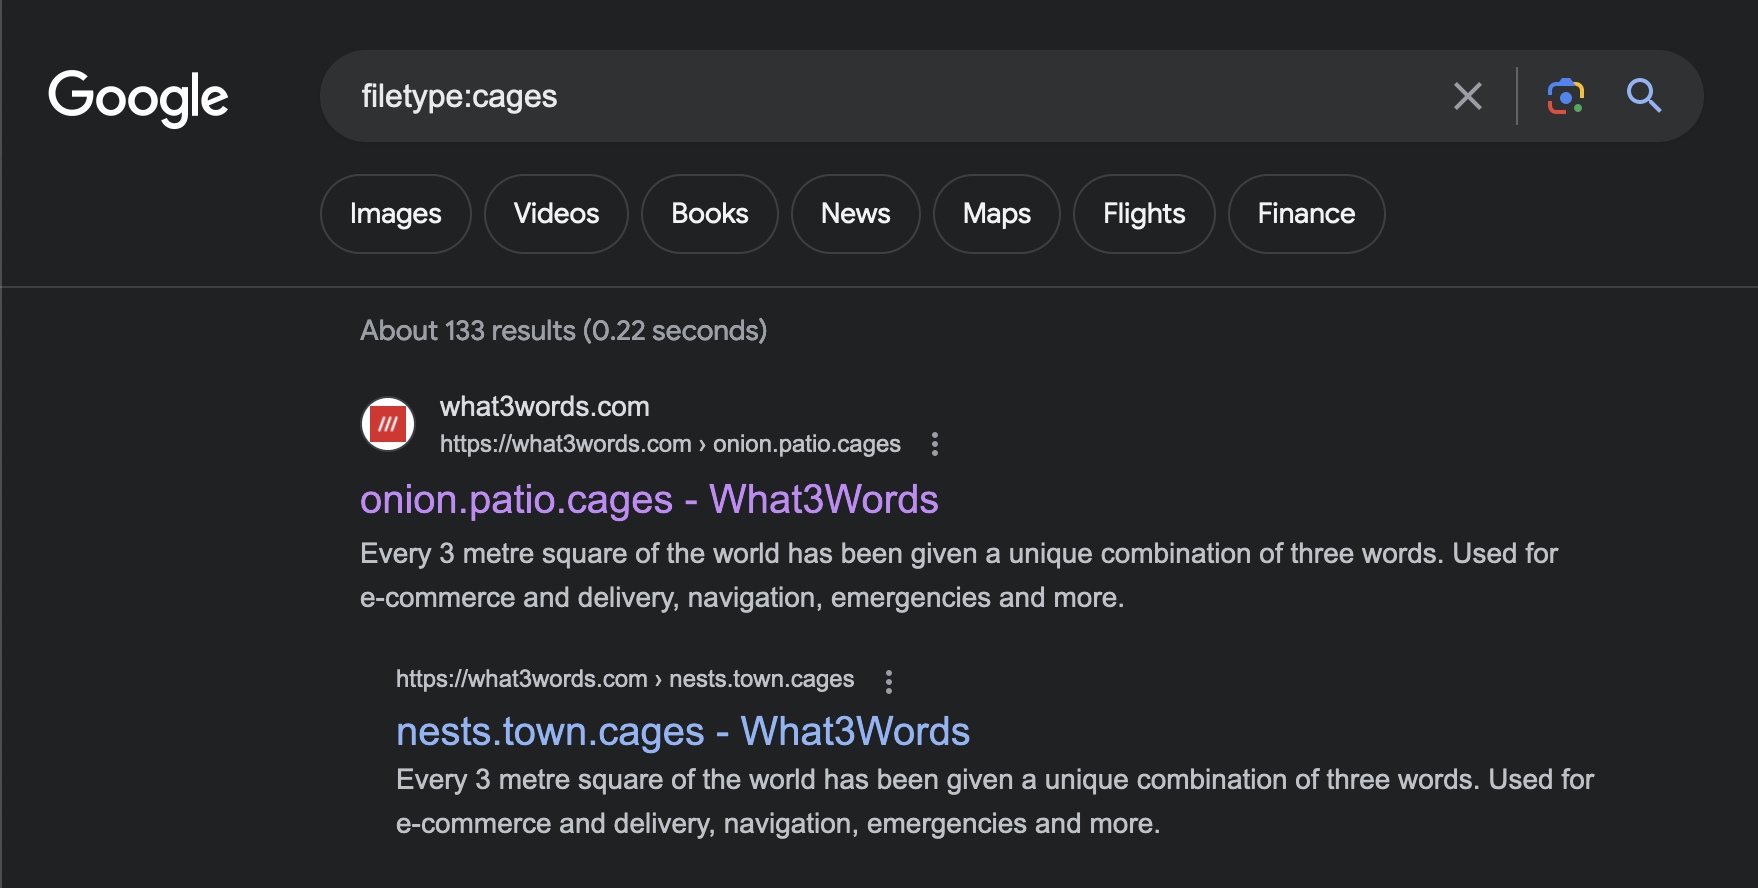
\includegraphics[width=15cm]{img/OSINT/The meeting/Skjermbilde 2023-08-28 kl. 13.04.36.png}

After that i just followed the link and found the location of the meeting.

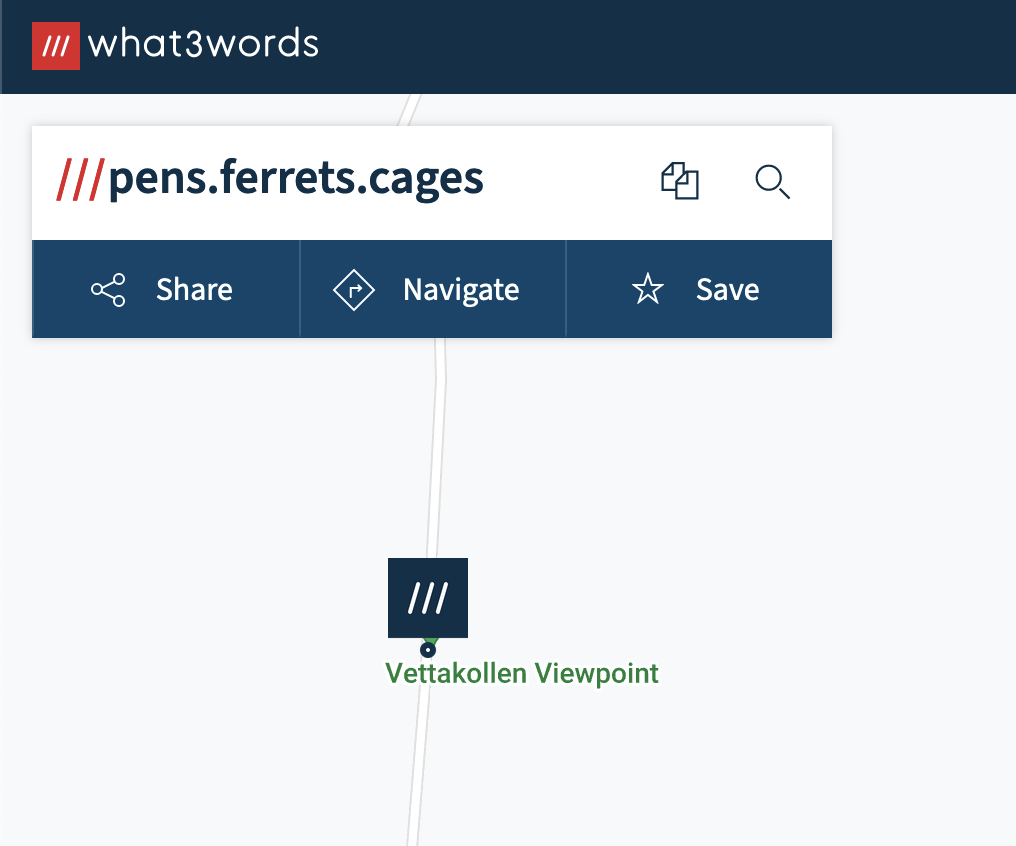
\includegraphics[width=10cm]{img/OSINT/The meeting/Skjermbilde 2023-08-28 kl. 13.03.54.png}

\subsection{Cherchez la femme (50p)}
I met this girl many years ago in Oslo. She was kind but very mysterious. She told me she lived in a hotel and wrote down her phone number on a piece of paper. She didn't even tell me her name and of course the phone number was fake. The same happens to me every time with girls with blue eyes :) After all these years can you help me to find her name at least?

\textbf{Solution:}\\
This task was pretty simple, all i did was to search the phone number from the image\dots

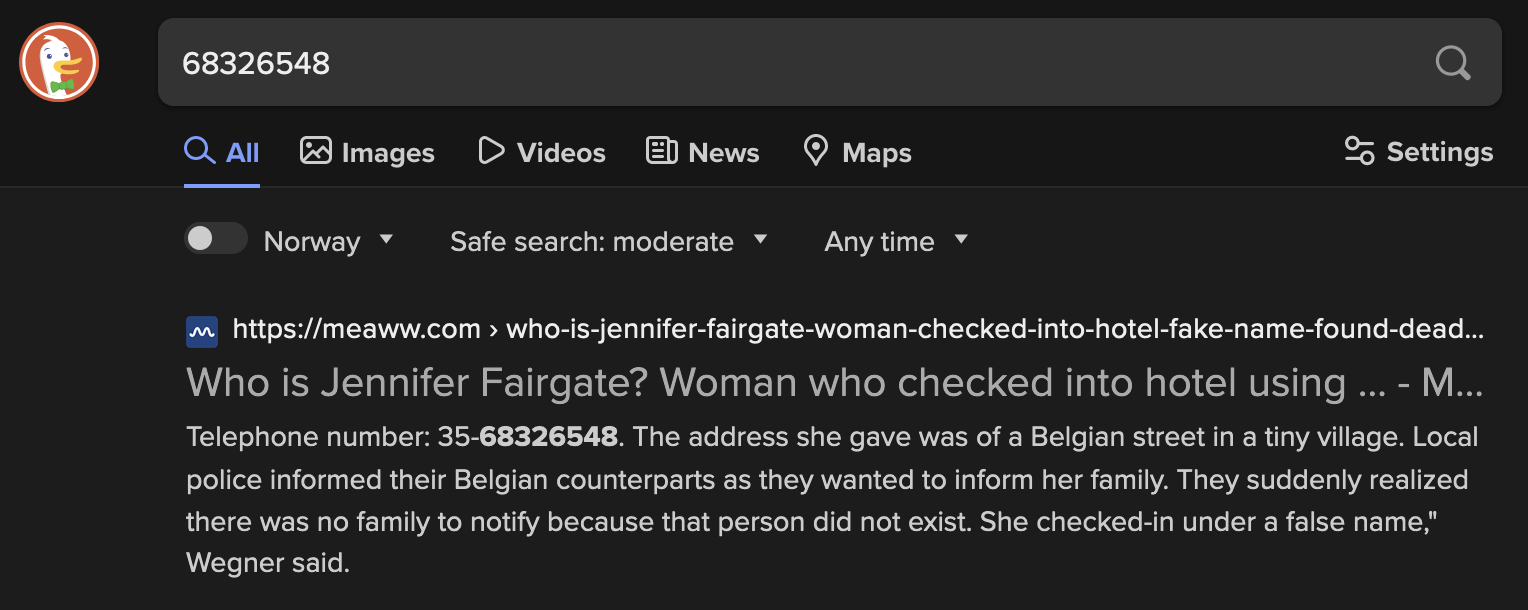
\includegraphics[width=12cm]{img/OSINT/Cherchez la femme/Skjermbilde 2023-08-28 kl. 11.55.32.png}

\dots and follow the link the the article\dots

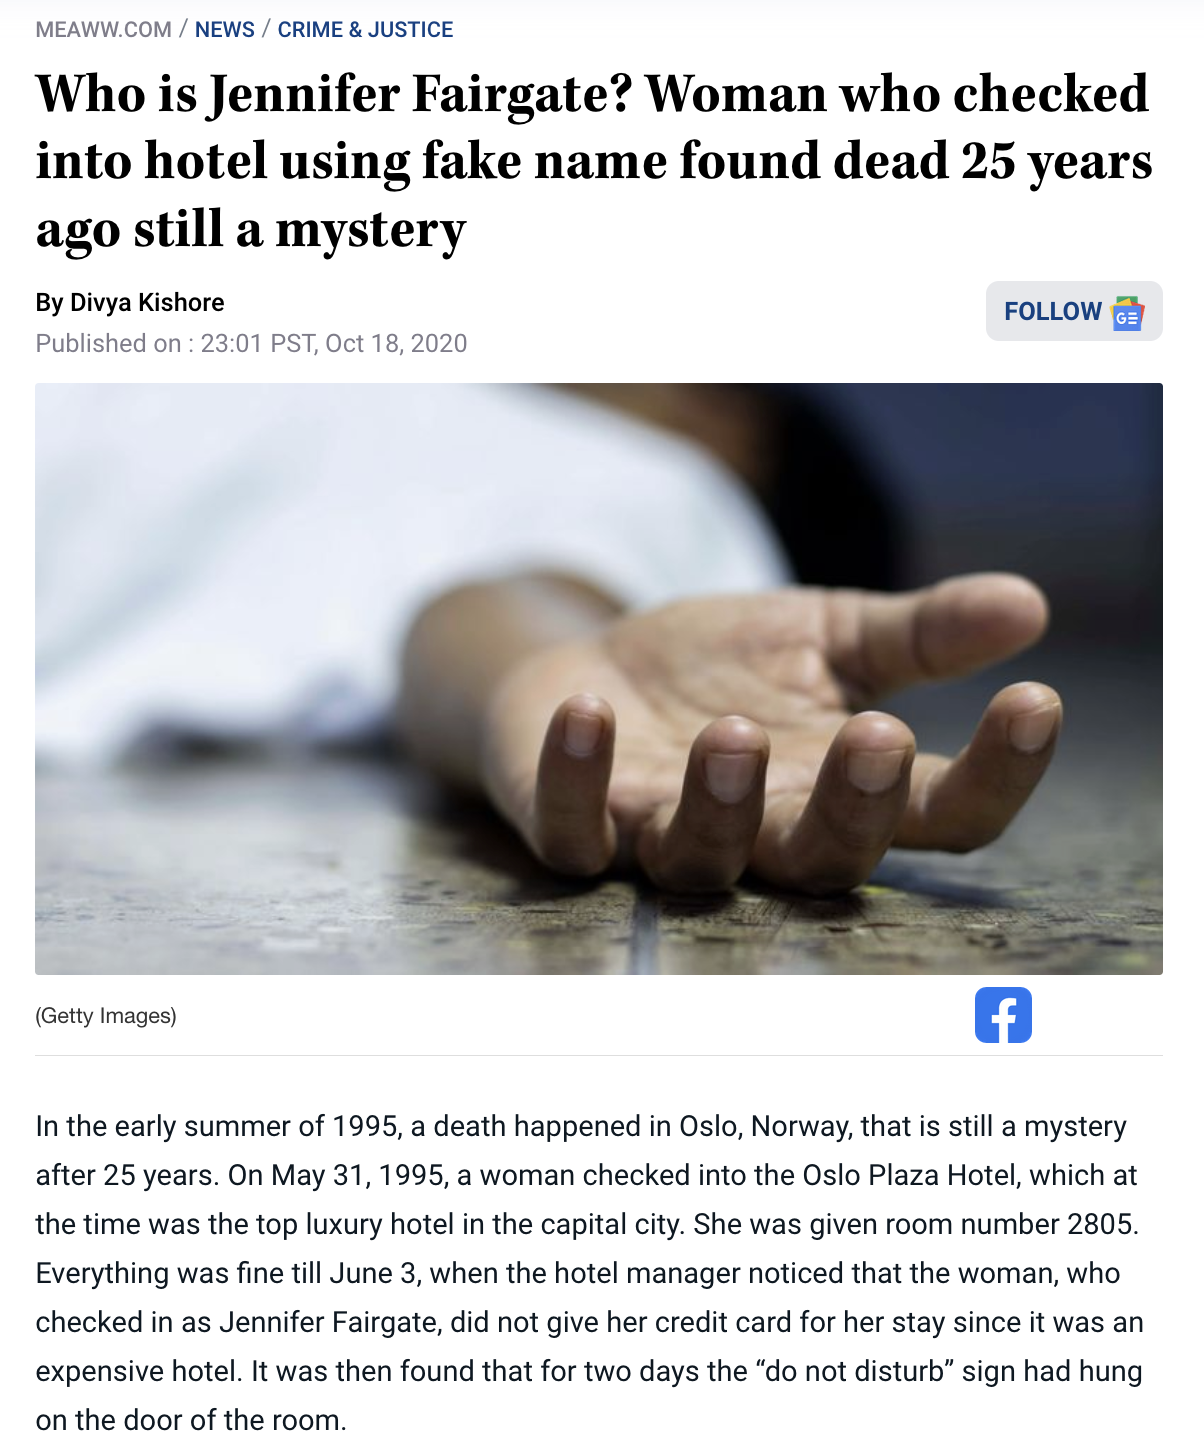
\includegraphics[width=10cm]{img/OSINT/Cherchez la femme/Skjermbilde 2023-08-28 kl. 11.56.40.png}

\dots to find the name.

\subsection{Quality software (50p)}
There's this software developer company the Quality Software Engineering Oslo. I think they stole our product code, so I need their Github password :)

\textbf{Solution:}\\
This task was a bit more difficult, mostly because I overlooked the results in the sidebar on Google. Regardless I managed to find the company on Google Maps.

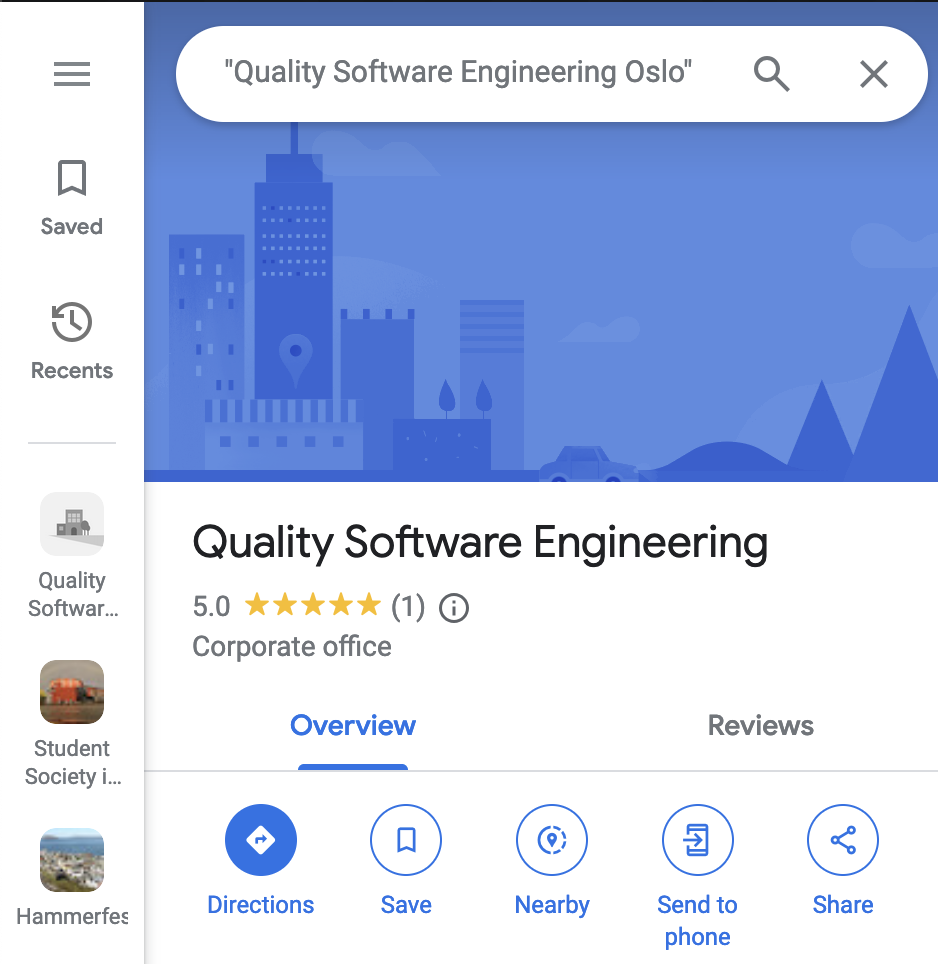
\includegraphics[width=7cm]{img/OSINT/Quality software/Skjermbilde 2023-09-11 kl. 17.30.32.png}

And found a review with an image.

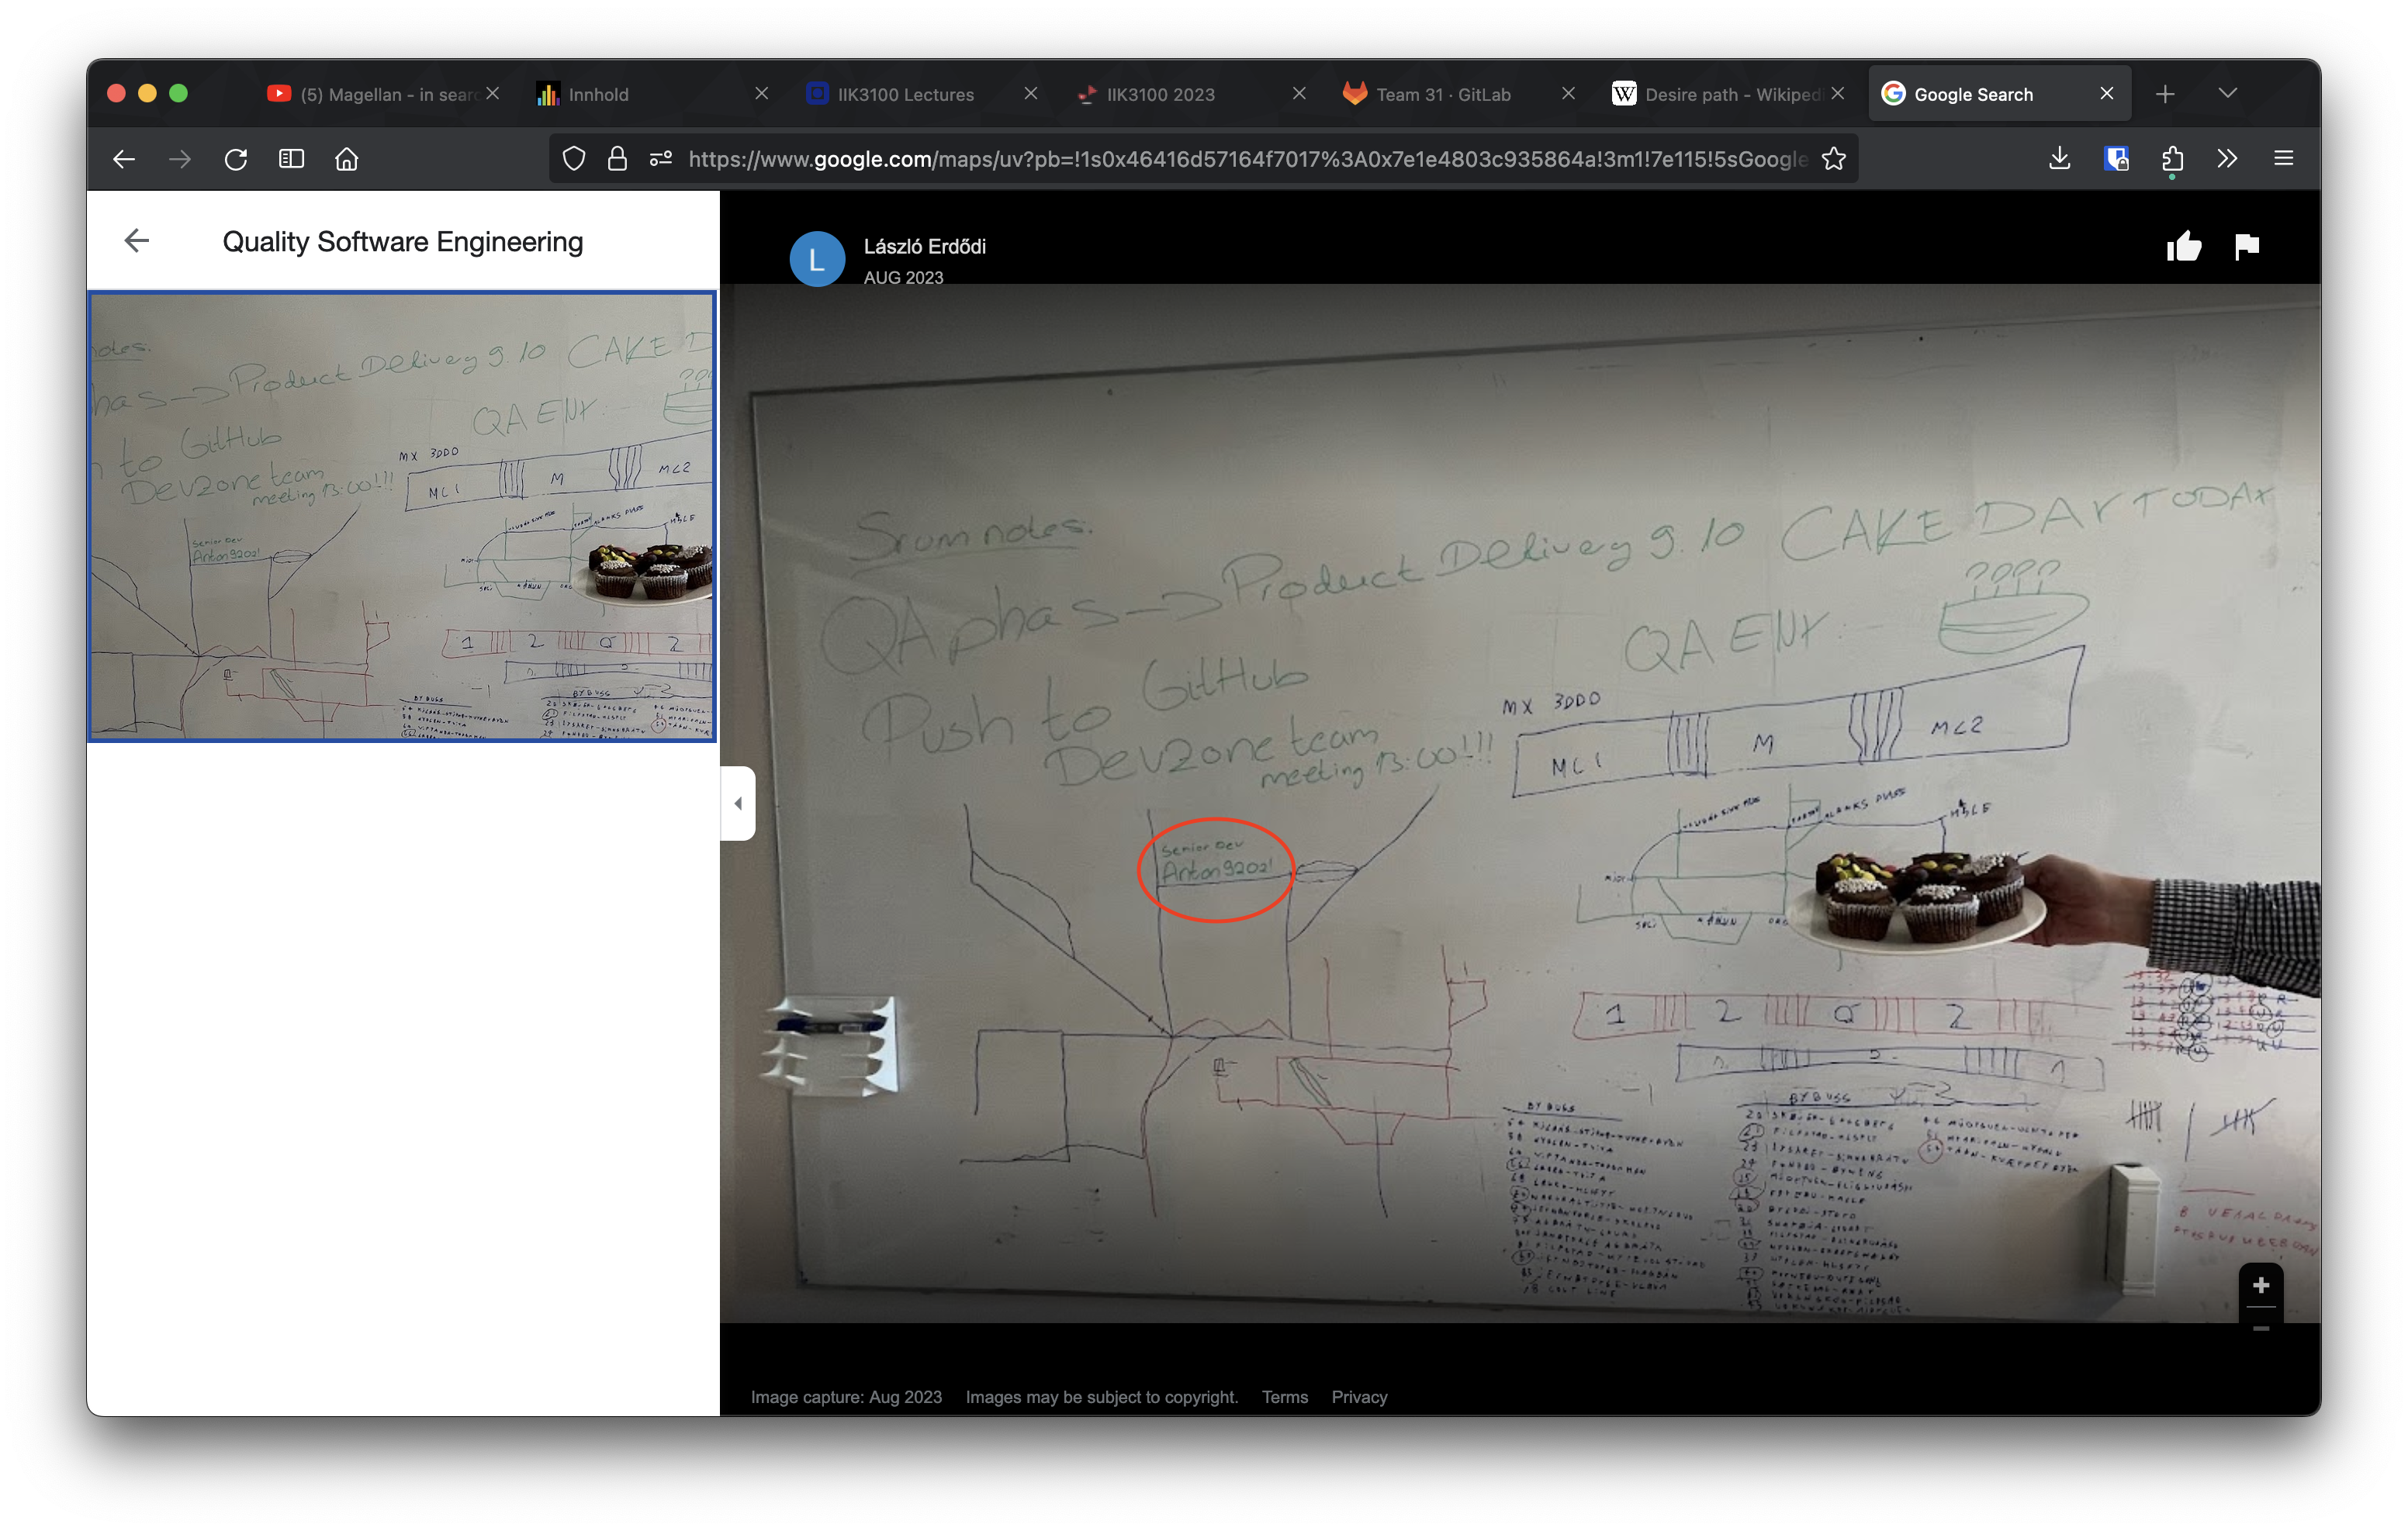
\includegraphics[width=16cm]{img/OSINT/Quality software/Skjermbilde 2023-09-06 kl. 11.54.53.png}

And after looking for a while I found a senior developer followed by a phrase that looked like a password.

\newpage
\subsection{The pitfall (80p)}
We captured one of them but we need a good answer to get the second one. The answer is the flag.
\begin{verbatim}
宏伟?
嗯
这是王林
非安全通道,少说信息
好
我们需要缺少那部分
周一9点,在奥斯陆Z地点
最后确认,谁在问?
\end{verbatim}

\textbf{Solution:}\\
The main challenge with this task was to translate the text correctly.
I first used Google Translate to translate the text, but didn't get any seemingly useful results when I searched with the translated text.
But using Yandex Translate I got that 宏伟 was a name, Hóngwěi, and 王林 was another name, Wáng lín.

\begin{center}
    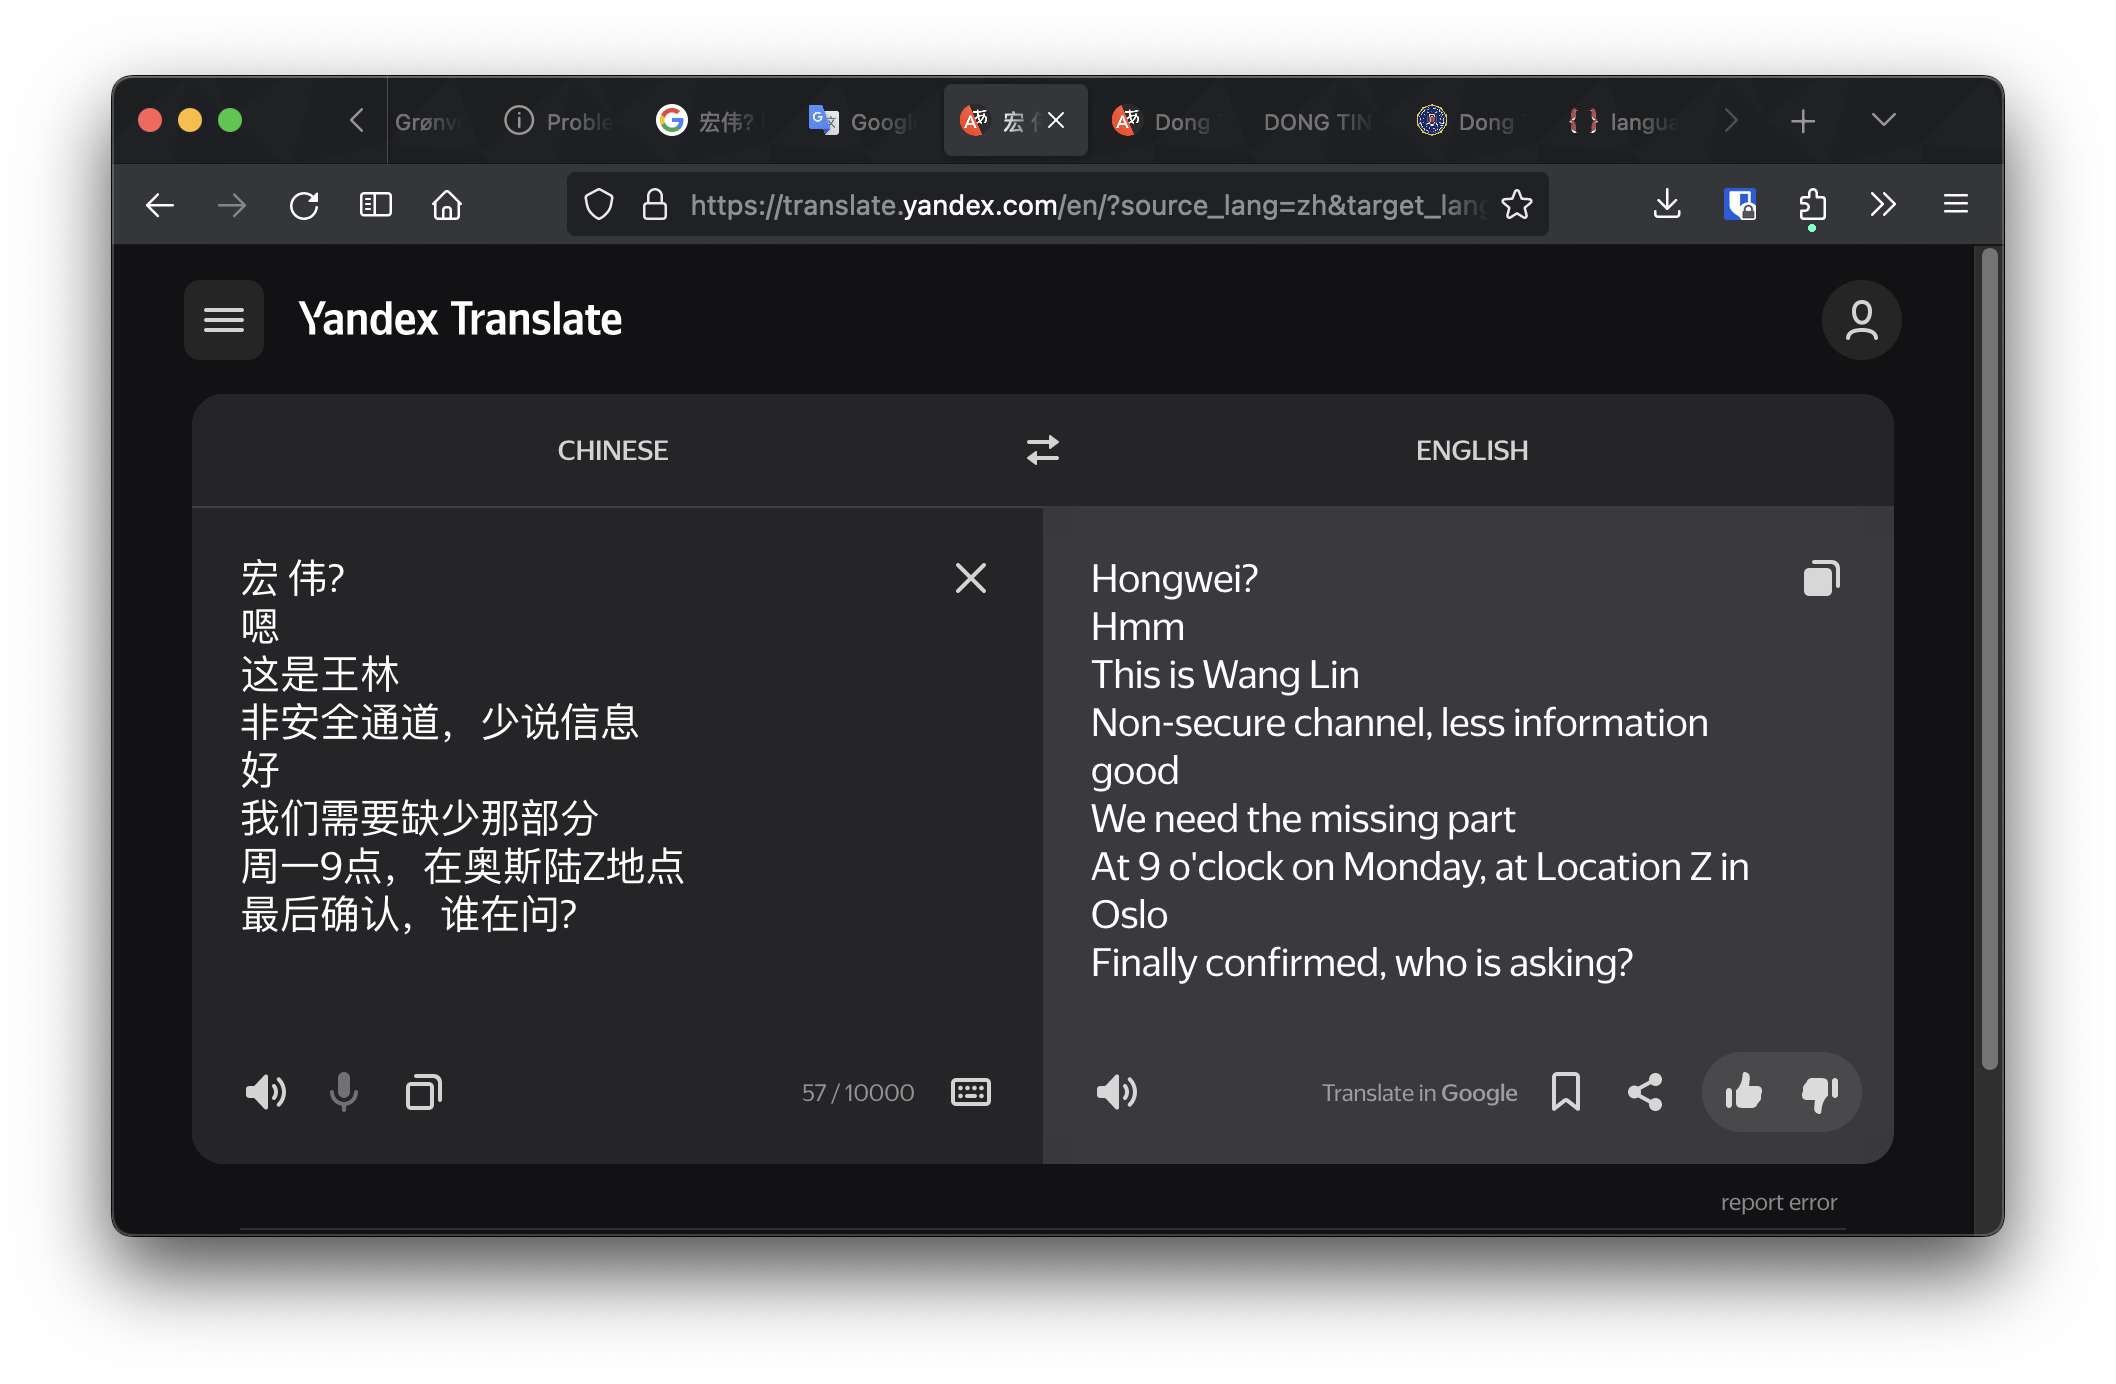
\includegraphics[width=16cm]{img/OSINT/The pitfall/Screenshot 2023-11-09 at 21.10.33.png}
\end{center}

Searching for the names resulted in an FBI listing with some other names as well, one of them being \texttt{Dong Ting}.

\begin{center}
    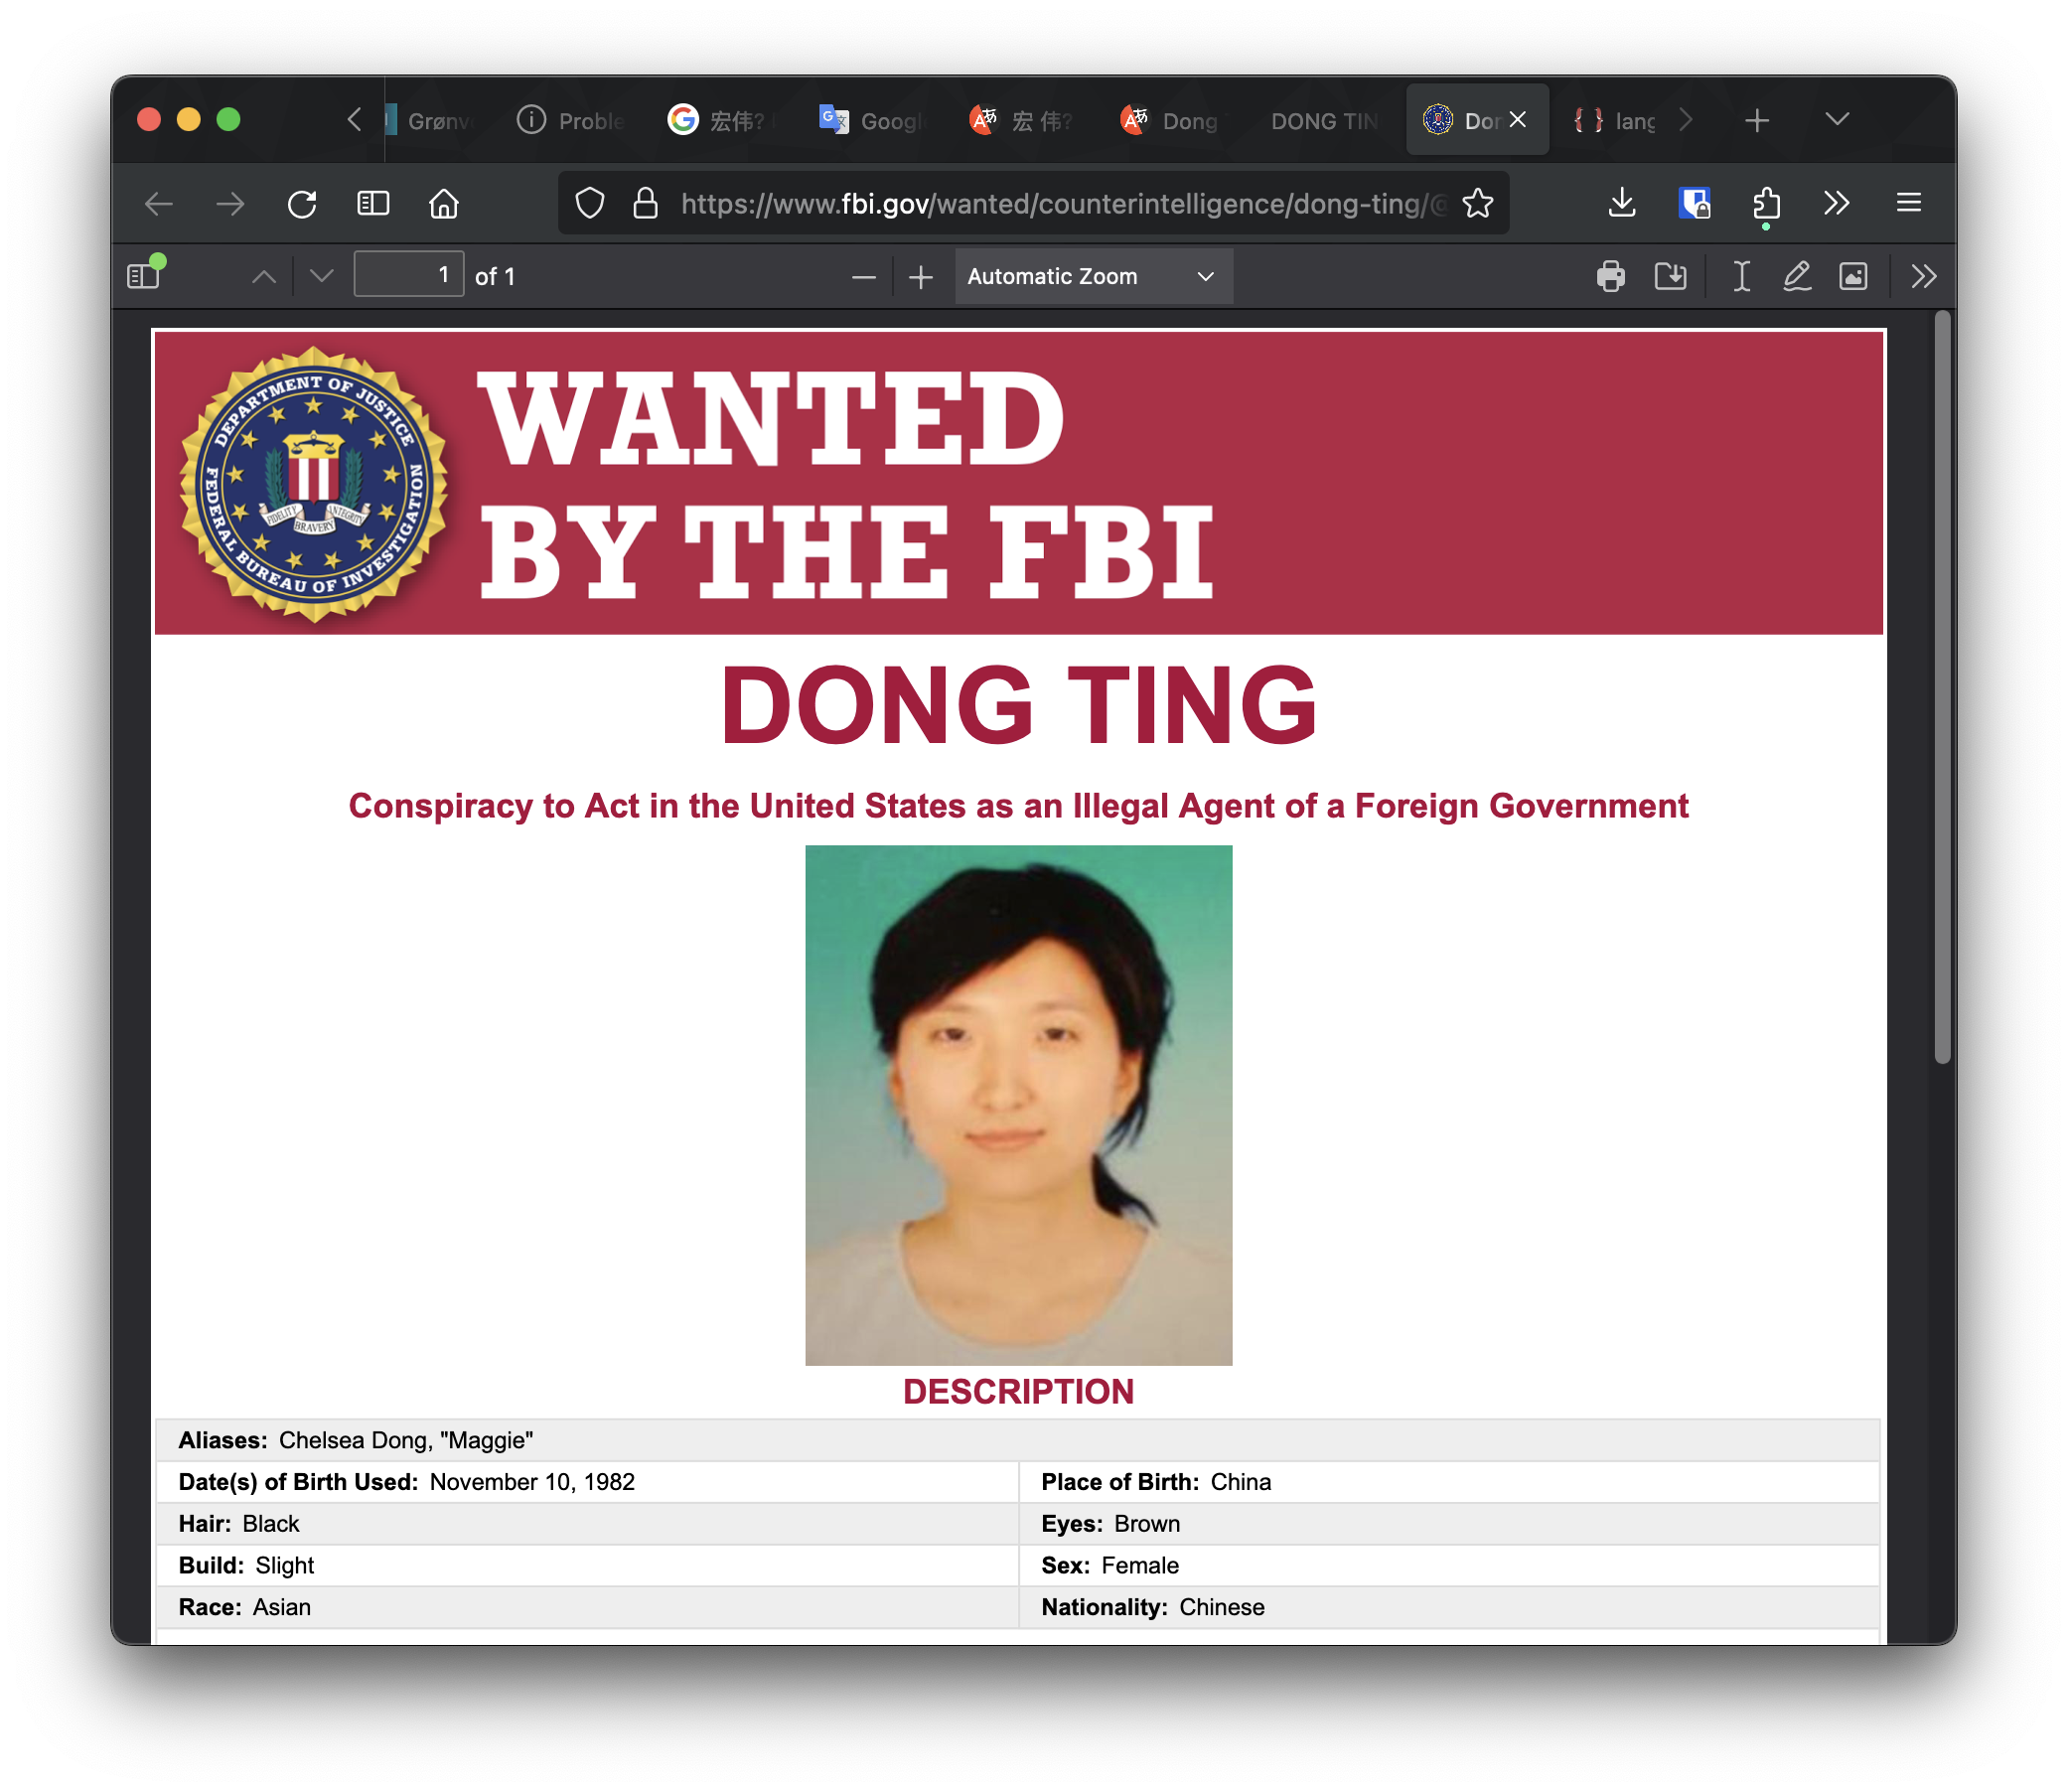
\includegraphics[width=12cm]{img/OSINT/The pitfall/Screenshot 2023-11-09 at 21.11.12.png}
\end{center}

Translating this to Chinese gave me \texttt{董婷} which was the answer.

\begin{center}
    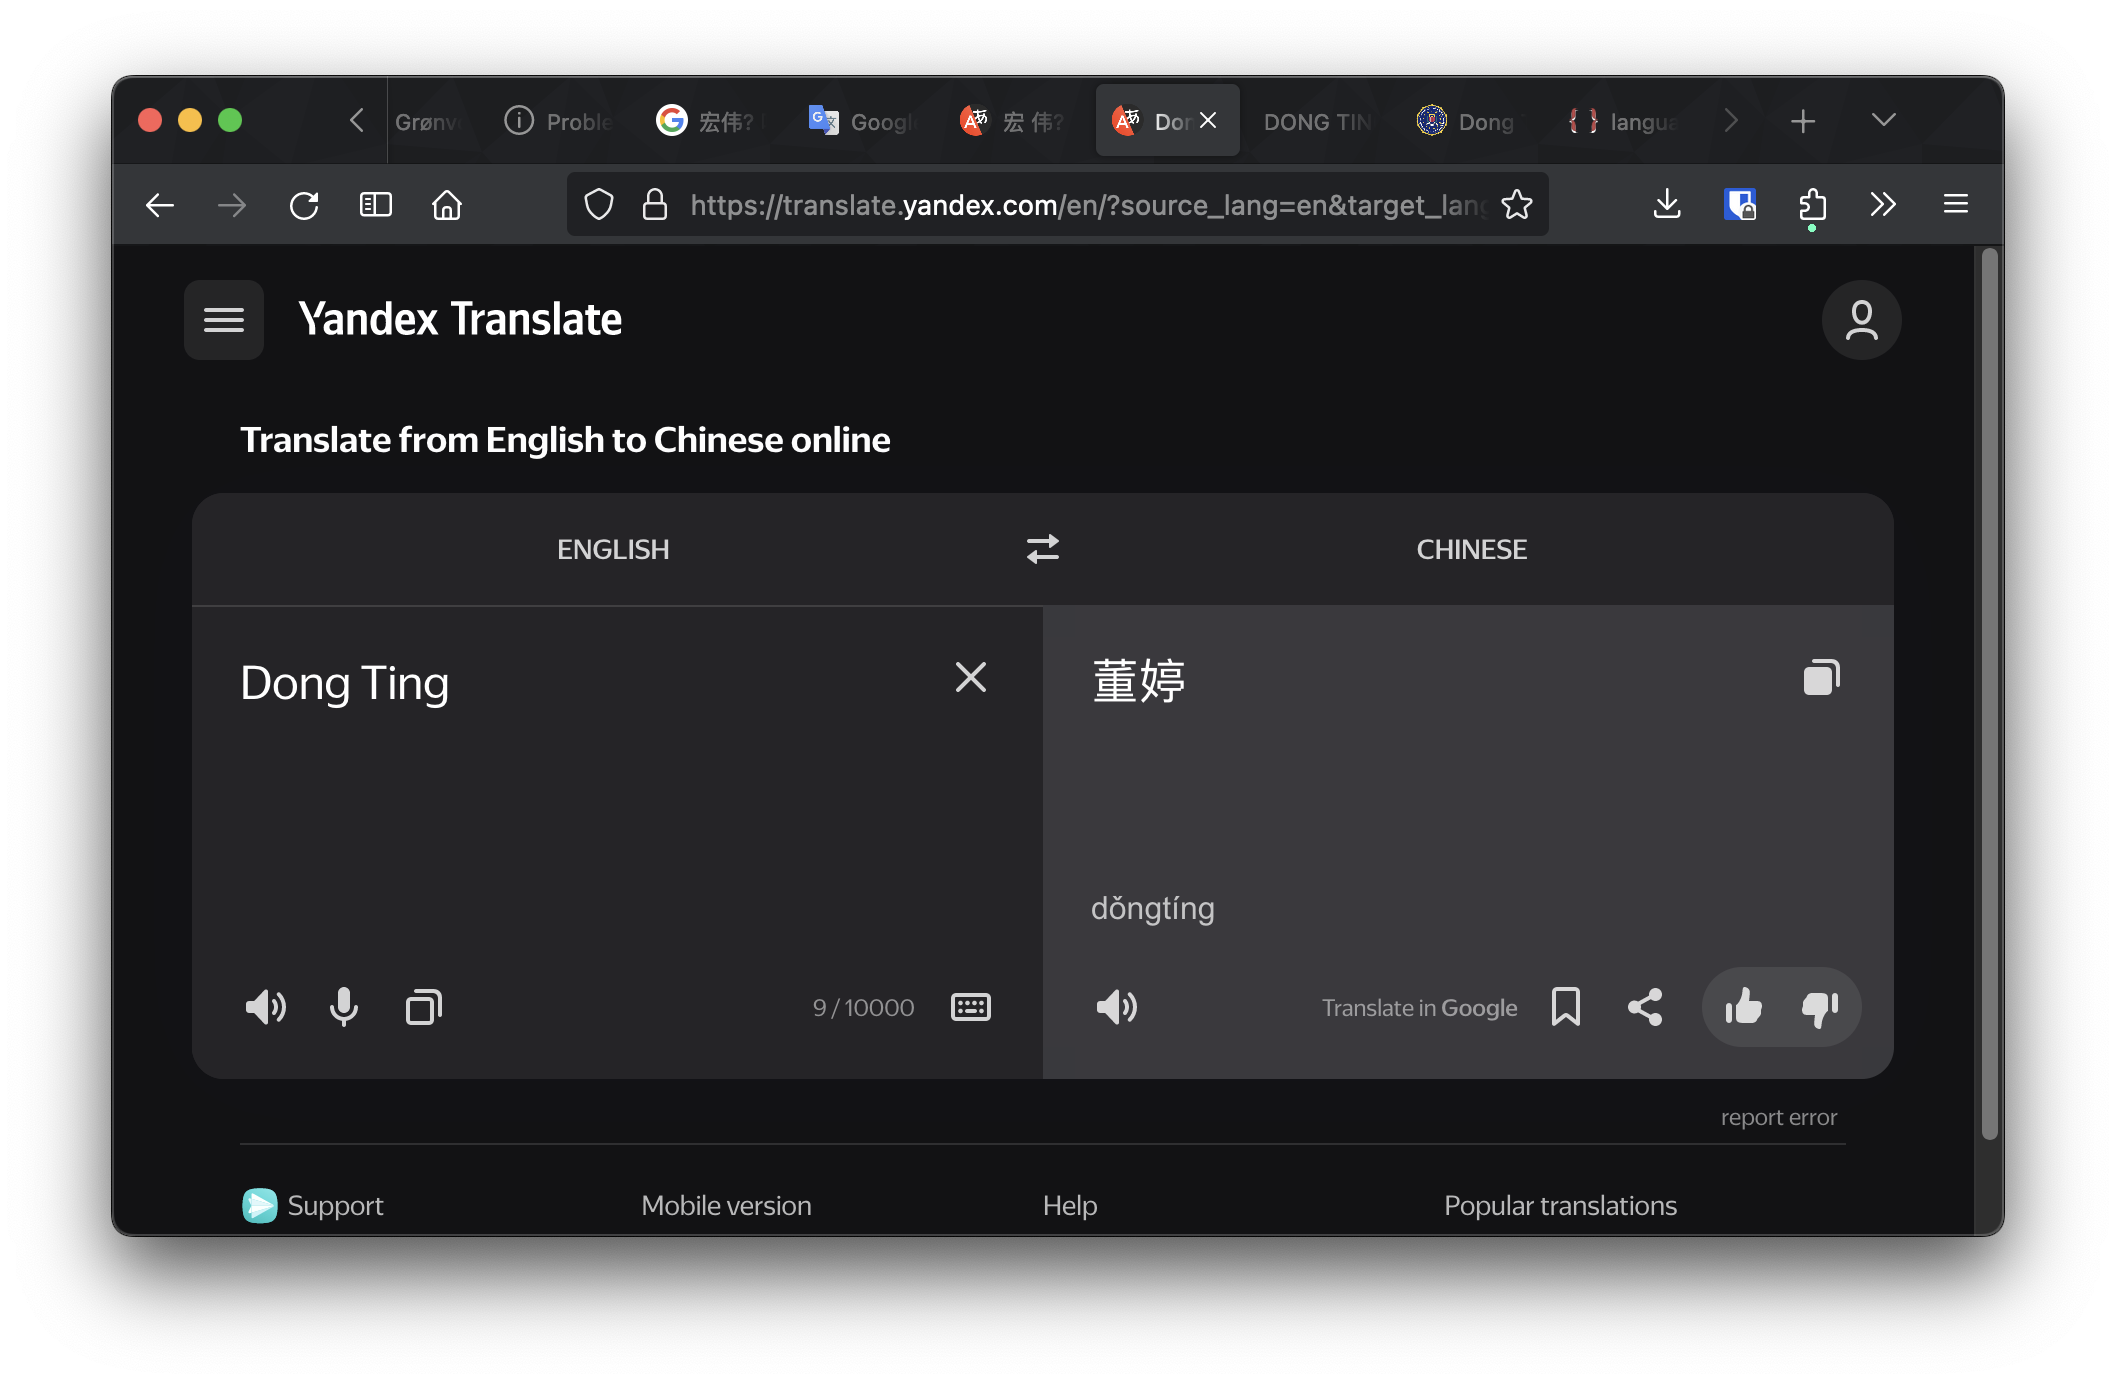
\includegraphics[width=14cm]{img/OSINT/The pitfall/Screenshot 2023-11-09 at 21.10.43.png}
\end{center}